\documentclass{article}

% PACKAGES  ============================================================
\usepackage{lipsum}		% Used to generate dummy-text (\lipsum[1])
\usepackage[margin=2.54cm,includefoot]{geometry}		% Used to control margins
\usepackage{scrextend}	% To be able to use \begin{addmargin}

\usepackage{graphicx} % allows to import images
\usepackage{float}	% allows for control of float positions
\usepackage{tikz} 	% Used to create trees, neural networks, 
\usetikzlibrary{matrix,chains,positioning,decorations.pathreplacing,arrows} % For neural networks

\usepackage{pgfplots}	% to create plots

\usepackage{forest} % Used to create trees

\usepackage{amsmath}	 % to use cases in equations and vectors

\usepackage[hidelinks]{hyperref}	% allows for clickable references

\usepackage[numbers,sort&compress]{natbib} 	% sorts the cites in increasing order automatically when referenced and compresses successive references

\usepackage[utf8]{inputenc}		% Be able to use umlaute

\usepackage[ngerman]{babel}

\usepackage{fancyhdr}	% Used for Header and Footer stuff

\usepackage{xfrac}	% allows for slanted fractions 

\usepackage{pgfplots}	% Used for function-plots


\usepackage{algorithm}		% Wirte pseudocode algorithms
\usepackage{algorithmic}

%\usepackage[table]  % Used for tables

% ============================================================

% HEADER AND FOOTER STUFF ============================================================
\pagestyle{fancy}
\fancyhead{}	% clears header
\fancyfoot{}	% clears footer
\fancyfoot[R]{\thepage}	% sets position right
\renewcommand{\headrulewidth}{0pt}	% removes header line by setting it to zero
\renewcommand{\footrulewidth}{1pt}		% add footer line by setting it to one
% ============================================================

% DEFINE LIST ITEM BULLETS ============================================================
\renewcommand{\labelitemi}{$\bullet$}	% first list item
\renewcommand{\labelitemii}{$\circ$}	% one-indented item
\renewcommand{\labelitemiii}{$\diamond$}	% twice-indented item
% ============================================================

% BE ABLE TO USE ROW AND COLUMN VECTORS INLINE ============================================================
\newcommand{\icol}[1]{% inline column vector
  \left(\begin{smallmatrix}#1\end{smallmatrix}\right)%
}

\newcommand{\irow}[1]{% inline row vector
  \begin{smallmatrix}(#1)\end{smallmatrix}%
}
% ============================================================


% TODO: Diese beiden sollten jeweils das \begin{flushleft} erstzen. 
% Jedoch ist der Text dann im Blocksatz, wenn flushleft fehlt...
%Einrücken von Absätzen deaktivieren
\setlength{\parindent}{0pt}
%Zeilenabstand bei Abstätzen
\usepackage{parskip}

\begin{document}

% TITLE PAGE ============================================================
\begin{titlepage}
	
	\begin{center}
	\line(1,0){330} \\
	[2mm]
	\huge{\bfseries Data Science Zusammenfassung} \\
	[2mm]
	\line(1,0){320} \\
	[1,5cm]
	\textsc{\LARGE By Yannis Schmutz} \\
	[0.75cm]
	\textsc{\large todo} \\
	
	\end{center}
	
\end{titlepage}
% ============================================================

% PREFACE STUFF ============================================================
\pagenumbering{roman}		% sets the page numbering to roman for the preface etc.
\section*{Zusammenfassung}	% Adds a section without a number in front
\addcontentsline{toc}{section}{\numberline{}Zusammenfassung}	% adds a section without a number in front to the ToC
\cleardoublepage	% Finishes the current page so that the following page will always be odd.
% ****************************************************************

% TABLE OF CONTENTS ============================================================
\renewcommand{\contentsname}{Inhaltsverzeichnis}	% Rename table of contents to the german version
\tableofcontents		% adds table of contents (this needs to be compiled twice sometimes in order to update)
\thispagestyle{empty}	% removes header & footer on this page
\cleardoublepage	% Finishes the current page so that the following page will always be odd.
% ============================================================

% LIST OF FIGURES ============================================================
%\renewcommand{\listfigurename}{Abbildungsverzeichnis}	% renames list of figures
\listoffigures	% generates a list of figures
\addcontentsline{toc}{section}{Abbildungsverzeichnis}	% Adds list of figures to the ToC
\cleardoublepage
% ============================================================

% LIST OF TABLES ============================================================
%\renewcommand{\listtablename}{Tabellenverzeichnis}
\listoftables
\addcontentsline{toc}{section}{Tabellenverzeichnis}
\cleardoublepage
% ============================================================

% START OF REGULAR CHAPTERS ============================================================
\setcounter{page}{1}		% Sets this page to the first one (and not the table of contents)
\pagenumbering{arabic}	% Sets the page numbering back to arabic

\newpage
\section{Einleitung}
\label{sec:stat}


blub äöü
\newpage
\section{Statistik}
\label{sec:stat}

\subsection{Begriffe}
\begin{flushleft}
Dieses Kapitel bietet eine grobe �bersicht �ber einige hilfreiche Begriffe der Statistik.

\subsubsection{Lageparameter}
Lageparameter beschreiben die Lage der Stichprobenelemente im Bezug auf die Messskala.
\linebreak

\textbf{Mittelwert} \\
Auch Durchschnitt (oder mean im Englischen) gennant. In der Wahrscheinlichkeitsrechnung spricht man oft vom Erwartungswert.

$$\bar{x}_{arithm} = \frac{1}{n} \sum_{i=1}^{n} x_i$$

\textbf{Median} \\ 
Der Median oder auch Zentralwert genannt, beschreibt den Wert aus der auf-/ absteigend geordneten Stichprobe, der genau in der Mitte liegt.

\begin{equation*}
  \widetilde{x} = \begin{cases}
    x_{\frac{n+1}{2}}, & \text{\textit{n} ungerade}\\
    \frac{1}{2} \left( x_{\frac{n}{2}} + x_{\frac{n}{1}+1} \right), & \text{\textit{n} gerade}.
  \end{cases}
\end{equation*}


\textbf{Quantile} \\
Schwellenwert (engl. percentile) der angibt, dass ein bestimmter prozentualer Wert einer Menge an Werten kleiner ist als das Quantil. 
Das Quantil bei 50\% ist der Median. Weitere spezielle Quantile sind die Quartile, die Quintile, die Dezile und die Perzentile.
\linebreak

\textbf{Modus} \\
Definiert den h�ufigsten Wert, der in der Stichprobe vorkommt.


\subsubsection{Streuungsparameter}
Streuungsparameter beschreiben die Streuung von Werten einer Stichprobe um einen bestimmten Lageparameter. So ergeben sich je nach gew�hlten Lageparameter unterschiedliche Berechungsformen. Diese unterscheiden sich in ihrer Beeinflussung durch Ausreisser. So wird beispielsweise der Median tendenziell weniger von einem einzelnen, sehr hohen Ausreisser beeinflusst als der arithmetische Mittelwert.
\linebreak

\textbf{Spannweite} \\
Die Spannweite (eng. range) gibt den Abstand des gr�ssten gegen�ber dem kleinsten vorkommenden Wert der Stichprobe an. $R = x_{max} - x_{min}$.
\linebreak
Die Spannweite wird stark durch Ausreisser beeinflusst. Dem kann jedoch durch das alternative Verwenden des \textbf{Interquartilsabstands} (engl. interquartile range) entgegengewirkt werden. Dieser berechnet n�mlich die Spannweite zwischen zwei Quantilen. Somit k�nnen Ausreisser ignoriert werden.
\linebreak

\textbf{Varianz} \\
\linebreak






\textbf{Korrelation}
\linebreak


\textbf{Kovarianz}
\linebreak


\textbf{Kausalit�t}
\linebreak


\end{flushleft}


% ****************************************************************
\newpage
\section{Probabilistik}
\subsection{Bedingte Wahrscheinlichkeit}

Die bedingte Wahrscheinlichkeit ist die Wahrscheinlichkeit des Eintreten eines Ereignisses A unter der Bedingung, dass die Wahrscheinlichkeit für das Eintreten eines Ereignisses B bereits bekannt ist. Man spricht von \dq{A} unter der Bedingung B\dq. Oder auch $P(A|B)$.\\


Sind zwei Ereignisse E, F voneinander \textbf{unabhängig}, so gilt:
$$ P(E \cap F) = P(E)P(F) $$
$$ P(E|F) = P(E)$$

Sind jedoch zwei Ereignisse A, B \textbf{nicht unabhängig} so lautet die Formel für A unter der Bedingung B:
	$$P(A|B) = \frac{P(A \cap B)}{P(B)}$$


Daraus erschliesst sich:
	$$P(A \cap B) = P(A|B)P(B)$$


Das Aufzeichnen eines Wahrscheinlichkeitsbaumes hilft zur Veranschaulichung: \\

\begin{figure}[H]
	\centering
	\label{fig:probability_tree}
	\begin{forest}
	%\label{fig:probability_tree}
	for tree={circle,draw, s sep=3em}
	[ 
	    [$B$,edge label={node[midway,left] {$P(B)$}}
	      [$A \cap B$,edge label={node[midway,left] {$P(A|B)$}} ] 
	      [$\bar{A} \cap B$,edge label={node[midway,right] {$P(\bar{A}|B)$}}] 
	    ]
	    [$\bar{B}$,edge label={node[midway,right] {$P(\bar{B})$}}
	      [$A \cap \bar{B}$, edge label={node[midway,left] {$P(A|\bar{B})$}}] 
	      [$\bar{A} \cap \bar{B}$, edge label={node[midway,right] {$P(\bar{A}| \bar{B})$}}] 
	  ] 
	]
	\end{forest}
	\caption{Wahrscheinlichkeitsbaum}
\end{figure}

\subsubsection{Satz von Bayes}
%Verweis auf Kapitel \pageref{sec:stat}.

Der Satz von Bayes zeigt den Zusammenhang zwischen $P(A|B)$ und $P(B|A)$ auf:

\begin{equation}
\label{eq:bayes_theorem}
	P(A|B) = \frac{P(A \cap B)}{P(B)} = \frac{P(B|A)P(A)}{P(B)}
\end{equation}

Diese Gleichung \ref{eq:bayes_theorem} entsteht, wenn man den Ausdruck $P(A \cap B)$ anhand den umgekehrten Wahrscheinlichkeitsbaums \ref{fig:inv_probability_tree} ausdrückt. 


\begin{figure}[H]
	\centering
	\label{fig:inv_probability_tree}
	\begin{forest}
	for tree={circle,draw, s sep=3em}
	[ 
	    [$A$,edge label={node[midway,left] {$P(A)$}}
	      [$A \cap B$,edge label={node[midway,left] {$P(B|A)$}} ] 
	      [$A \cap \bar{B}$,edge label={node[midway,right] {$P(\bar{B}|A)$}}] 
	    ]
	    [$\bar{A}$,edge label={node[midway,right] {$P(\bar{A})$}}
	      [$\bar{A} \cap B$, edge label={node[midway,left] {$P(B|\bar{A})$}}] 
	      [$\bar{A} \cap \bar{B}$, edge label={node[midway,right] {$P(\bar{B}| \bar{A})$}}] 
	  ] 
	]
	\end{forest}
	\caption{Umgekehrter Wahrscheinlichkeitsbaum}
\end{figure}
% ****************************************************************



% ****************************************************************
\newpage
\section{Feature Scaling}

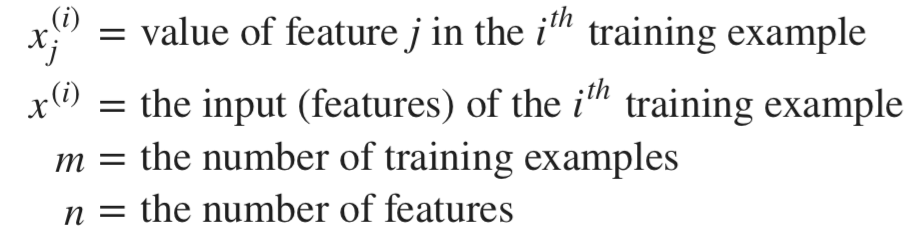
\includegraphics[scale=0.5]{figures/feature_notation}

\subsection{Mean normalization}

$$ x_{j} = \frac{x_{j}^{i} - \mu_{j}}{max(x_{j}) - min(x_{j})} \qquad\forall x^{i} \in x_{j}$$

% ****************************************************************
% ****************************************************************
\newpage
\section{Machine Learning}
\label{sec:ml}

\subsection{Übersicht}

\begin{figure}[H]
	\centering
	\label{fig:ml_overview}
	\begin{forest}
	for tree={draw, s sep=3em}
	[Machine Learning
	    [Überwachtes Lernen
	        [Klassifizierung
	            [Naive Bayes]
	             [k-N-N]
	             [NN]
	        ]
	        [Regression
	            [Linear Regression]
	            [NN]
	        ]
	    ]
	    [Unüberwachtes Lernen
	        [Clustering
	            [K-means]
	        ]
	        [Assoziierung]
	    ]
	]
	\end{forest}
	\caption{Machine Learning Kategorien}
\end{figure}

% #################################
\subsubsection{Überwachtes Lernen}
\begin{flushleft}

Überwachte Lern-Algorithmen probieren Beziehungen und Abhängigkeiten zwischen den Input-Features und des zu erzielenden Outputs zu erschliessen. Dies unter der Verwendung von \textbf{beschrifteten Daten}. Diese können zu Trainingszwecken verwendet werden. Jeder Satz an Daten besteht aus Input-Werten sowie einem dazugehörigen bekannten Output-Wert. Nach dem Trainieren des Algorithmus versucht dieser anhand von \textbf{neuen} Input-Features den dazugehörigen \textbf{unbekannten} Output vorherzusagen.
\linebreak

Das überwachte Lernen kann in zwei Kategorien unterteilt werden:

\begin{itemize}
	\item \textbf{Klassifizierung:} Ziel der Klassifizierung ist es, diskrete Werte vorherzusagen (bspw. Wahr/ Falsch, Spam-Mail/ normales Mail). 
	\item \textbf{Regression:} Das Ziel der Regression ist die Vorhersage kontinuierlicher Werte (bspw. Hauspreise in Abhängigkeit von Flaeche und Anzahl Zimmer).
\end{itemize}

\end{flushleft}

\subsubsection{Unueberwachtes Lernen}
\begin{flushleft}

Im unüberwachten Lernen stehen den Algorithmen \textbf{keine} beschrifteten Daten zur Verfügung. Die Algorithmen versuchen eigenständig Pattern in den zu behandelnden Daten zu erkennen und sie dadurch beispielsweise gruppieren zu können.
\end{flushleft}

% #################################

% ****************************************************************



% ****************************************************************
\newpage
\section{Gradient Descent}

\begin{flushleft}

Gradient Descent ist ein Optimierungsalgorithmus, um ein lokales Minimum einer Funktion zu finden.
Gegeben sei eine Kosten-Funktion $J(\Theta_{0}, \Theta_{1})$, gesucht ist das Minimum der Funktion $min_{\Theta_{0}, \Theta_{1}} J(\Theta_{0}, \Theta_{1})$, indem die Parameter $\Theta_{0}$ und $\Theta_{0}$ laufend ein wenig verändert werden.

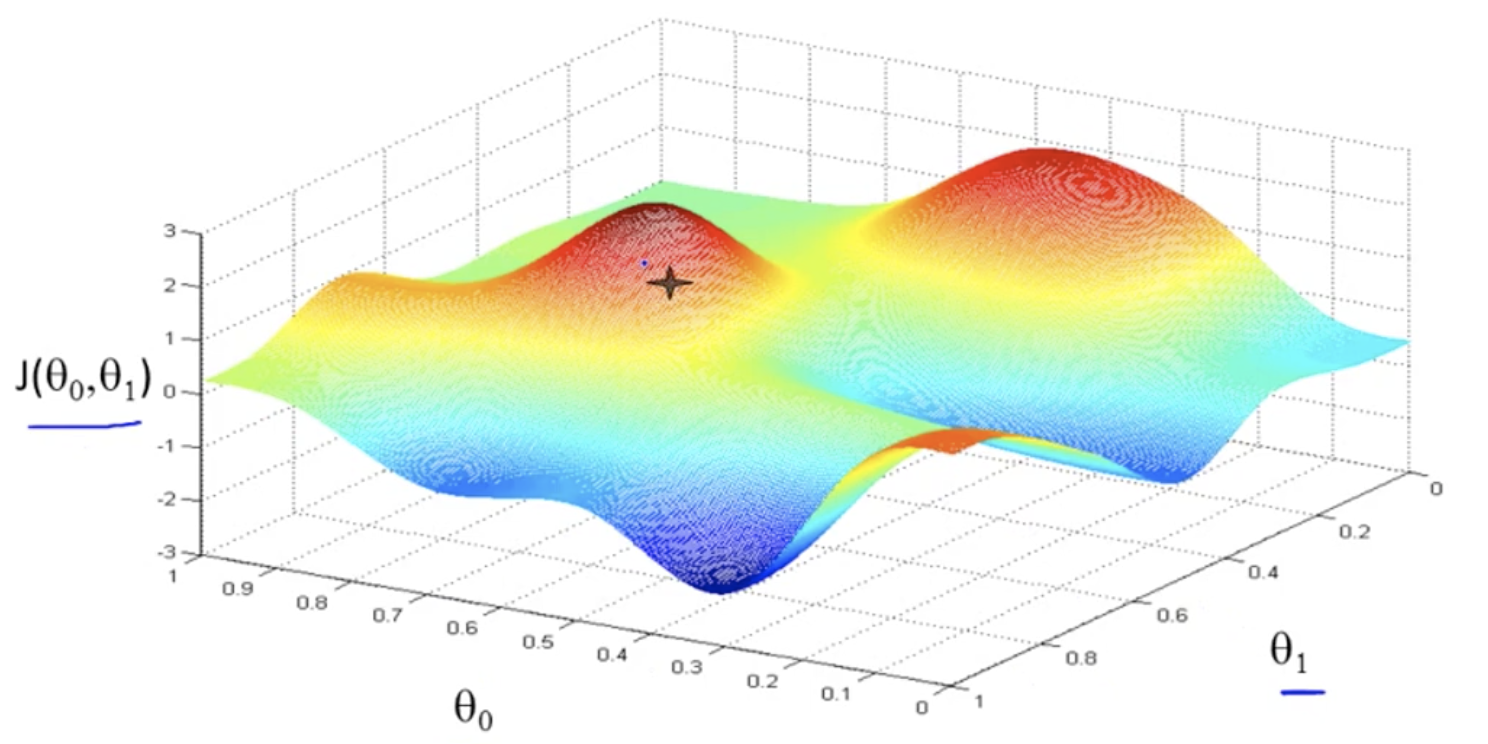
\includegraphics[scale=0.6]{figures/gradient_descent}

Wiederholen bis zur Konvergenz:
$$\Theta_{i} := \Theta_{i} - \alpha\frac{\partial}{\partial \Theta_{i}} J(\Theta_{0}, \Theta_{1}) $$

$$ \alpha: Learning Rate $$
$$ i=0, i=1 $$

\subsubsection{GD für Linear Regression}
Model Funktion:
$$h_{\Theta} = \Theta_{0} + \Theta_{1}x$$
Cost-Function:
$$ J(\Theta_{0}, \Theta_{1}) = \frac{1}{2m} \sum_{i=1}^{m}(h_{\Theta}(x^{(i)})-y^{(i)})^{2} $$

Für lineare Regression hat die Kostenfunktion stets nur ein lokales (sprich globales) Minimum.
\linebreak
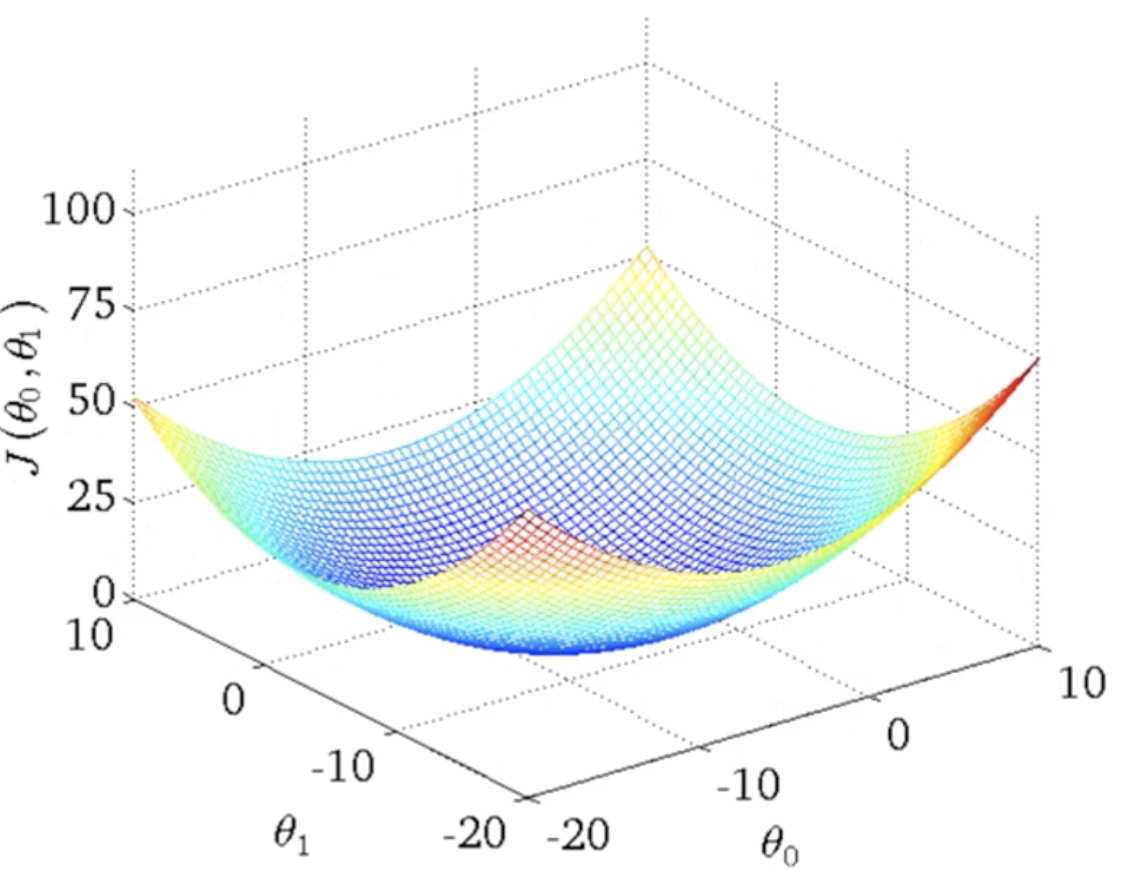
\includegraphics[scale=0.6]{figures/cost_function_linear_regression}
\linebreak
Der Gradient Descent Algorithmus für eine simple Lineare Regression rechnet sich wie folgt:
\linebreak


\begin{algorithm}
\caption{Calculate $\text{min}_{\Theta} J(\Theta)$}
\begin{algorithmic} 
\REPEAT 
\STATE $ \Theta_{0} := \Theta_{0} - \alpha \frac{1}{m} \sum_{i=1}^{m}(h_{\Theta}(x^{(i)}) - y^{(i)}) $

\STATE $ \Theta_{1} := \Theta_{1} - \alpha \frac{1}{m} \sum_{i=1}^{m}(h_{\Theta}(x^{(i)}) - y^{(i)})*x^{(i)} $
\COMMENT{simultaneously update all $\Theta_{j}$}
\UNTIL{$J(\Theta_{0}, \Theta_{1})$ converges}
\end{algorithmic}
\end{algorithm}


\end{flushleft}
% ****************************************************************




\newpage
\section{Normal Equation}
\begin{flushleft}

Die Normal Equation ist eine Alternative zum Gradient Descent und rechnet sich wie folgt:

$$ \Theta = (X^{T}X)^{-1}X^{T}y $$

Unterschied zu Gradient Descent:
\begin{table}[h]
	\begin{tabular}{|l|l|}
		\hline
		{\textbf{Gradient Descent}} 		& {\textbf{Normal Equation}} 		\\ \hline
		Alpha muss gewählt werden       & Alpha muss nicht gewählt werden   \\ \hline
		Benötigt viele Iterationen      & Benötigt keine Iterationen        \\ \hline
		$O(kn^{2})$                     & $O(n^{3})$                        \\ \hline
		Auch für grosses n performant   & Langsam für grosses n             \\ \hline
	\end{tabular}
\end{table}
\end{flushleft}

\newpage
\section{Linear Regression}
\begin{flushleft}

Die lineare Regression ist ein Verfahren welches versucht, eine abhängige Variable durch eine oder mehrere unabhängige Variablen zu erklären.

\subsection{Simple lineare Regression}

Die simple lineare Regression arbeitet lediglich im zweidimensionalen Raum.

\begin{tikzpicture}
\begin{axis} [
	axis lines = left, % Only displays axis on left and bottom (not whole box)
	ymin = 0,	% y-axis shall always start at zero
	xlabel = $x$,
	ylabel = $f(x)$,
	mark=*,
	scatter/classes={%	Defines the point appearance for the scatter plot
		a={blue}%,
		%b={mark=triangle*,red},
		%c={mark=o,draw=black}
		}
	]

\addplot [
	domain = 0:60, 	% Range for the value x
	samples = 100,	% Determines the number of points in the interval defined by domain. 
	color = red,	% Color of the
	] {0.83*x + 10.44};
\addlegendentry {$mx + q$}

\addplot [only marks, scatter, scatter src=explicit symbolic]
	table [meta=class] {		% meta defines the column to use for the class of the point
		x		y		class
		10		20		a
		10		15		a
		15		17		a
		20		21		a
		20		31		a
		25		40		a
		30		27		a
		35		40		a
		30		55		a
		40		45		a
		40		37		a
		45		52		a
		50		55		a
		50		45		a
		55		50		a
		60		65		a
		
	};

\end{axis}
\end{tikzpicture}

Die Steigung [m] sowie der y-Achsenabschnitt [q] lassen sich wie folgt berechnen:

$$m = \dfrac{\sum_{i=1}^n (x_{i} - \bar{x})(y_{i} - \bar{y})}
                       {\sum_{i=1}^n (x_{i} - \bar{x})^{2}}$$

$$q = \bar{y} - m\bar{x}$$

Wobei die werte $\bar{x}$, $\bar{y}$ den arithmetischen Mitteln der Definitions- und Bildmenge entsprechen.
\linebreak
Die Qualität eines Regressionsmodells kann durch Genauigkeitsmetriken bestimmt werden. Hierbei werden stets die effektiven Y-Werte mit den jeweiligen Werten $\hat{y}_{i} = mx_{i} + q$ der linearen Regressionslinie verglichen.


Der \textbf{Mittlerer absoluter Fehler} (mean-absolute-error) ist die simpleste Metrik und zeig den effektiven Durchschnittsfehelr auf. 
$$MAE = \dfrac{1}{n}\sum_{i=1}^n|y_{i} - \hat{y}_{i}|$$


Die \textbf{Mittlere quadratische Abweichung} (mean-square-error) reagiert aufgrund des Exponenten proportional stärker auf grosse Fehler.
$$MSE = \dfrac{1}{n}\sum_{i=1}^n(y_{i} - \hat{y}_{i})^{2}$$

Der \textbf{root-mean-square-error} ist die gängigste Metrik, da dieser, durch das Ziehen der Wurzel, in der gleichen Einheit interpretierbar ist wie die eigentlichen Y-Vektoren.
$$RMSE = \sqrt{\dfrac{1}{n}\sum_{i=1}^n(y_{i} - \hat{y}_{i})^{2}} = \sqrt{MSE}$$


\subsection{Polynomial Regression}
\subsection{Multivariable Regression}

\end{flushleft}
\newpage
\section{Logistic Regression}
\subsection{Binary classification}
\begin{flushleft}


Mittels Logistischer Regression lassen sich diskrete Phänomene klassifizieren. Die Funktion des Models ist wie folgt definiert:


$$ h_{\Theta}(x) = g(\Theta^{T}x) $$ 
x ist hierbei lediglich der Featurevektor eines Samples $\icol{x_{1}\\x_{2}\\x_{3}}$. Eine vektorielle Implementation für alle Featuresamples (Matrix) ist weiter unten beschrieben.
$$ g(z) = \frac{1}{1 + e^{-z}} $$
$$ h_{\Theta}(x) = \frac{1}{1 + e^{-\Theta^{T}x}} $$

Die Funktion $g(x)$ ist hierbei die sogenannte Sigmoid (oder auch logistische) Funktion.

\begin{tikzpicture}[declare function={sigma(\x)=1/(1+exp(-\x));}]
\begin{axis}%
[
    grid=major,     
    xmin=-8,
    xmax=8,
    axis x line=bottom,
    ytick={0,.5,1},
    ymax=1,
    axis y line=middle,
    samples=100,
    domain=-8:8,
    legend style={at={(1,0.9)}}     
]
    \addplot[blue,mark=none]   (x,{sigma(x)});
    \legend{$g(x)$}
\end{axis}
\end{tikzpicture}

Der Wert $h_{\Theta}(x)$ wird als Wahrscheinlichkeit verstanden, dass der Output (y) positive ist für ein gegebener Eingabewert (x) parametrisiert mit $\Theta$.
\linebreak

Formal definiert:
$$h_{\Theta}(x) = P(y=1|x;\Theta)$$
Somit gilt:
$$ P(y=0|x;\Theta) = 1 - P(y=1|x;\Theta)$$



Cost-Function:

$$ J(\Theta) = \frac{1}{m}\sum_{i=1}^{m}Cost(h_{\Theta}(x^{(i)}), y^{(i)}) $$


$$ \text{Cost}(h_{\Theta}(x), y) =
    \begin{cases}
      -\text{log}(h_{\Theta}(x)) & \text{for } y=1\\
      -\text{log}(1 - h_{\Theta}(x)) & \text{for } y=0\\
    \end{cases} $$

Im Gegensatz zur linearen Regression wird bei der logistischen die Cost-Funktion je nach Fall (Wert von y) unterschieden, um eine konvexe Funktion zu generieren.
Graphisch dargestellt sieht die Cost-Function wie folgt aus:

\begin{tikzpicture}[declare function={c1(\x)=-log2(x); c0(\x)=-log2(1-x);}]
\begin{axis}%
[
    grid=major,     
    xmin=-0.1,
    xmax=1,
    axis x line=bottom,
    ytick={0,1,2,3,4,5},
    ymax=5,
    axis y line=middle,
    samples=1000,
    domain=0:1,
    legend style={at={(1,0.9)}}     
]
    \addplot[blue,mark=none]   (x,{c1(x)});
    \addplot[red,]   (x,{c0(x)});
    \legend{$\text{cost1}(x)$, $\text{cost0}(x)$}
\end{axis}
\end{tikzpicture}


\begin{algorithm}
\caption{Calculate $\text{min}_{\Theta} J(\Theta)$}
\begin{algorithmic} 
\REPEAT 
\STATE $ \Theta_{j} := \Theta_{j} - \alpha\sum_{i=1}^{m}(h_{\Theta}(x^{(i)}) - y^{(i)})x_{j}^{(i)} $
\COMMENT{simultaneously update all $\Theta_{j}$}
\UNTIL{$J(\Theta)$ converges}
\end{algorithmic}
\end{algorithm}

Eine Vektor-Implementation dieses Algorithmus sieht so aus:

$$ \Theta := \Theta - \frac{\alpha}{m} X^{T}(g(X\Theta) - \vec{y}) $$

\subsubsection{Regularization}

TODO


% ****************************************
\subsection{Multiclass classification}
\subsubsection{One-vs-all}

Sei $y = {0, 1, ..., n}$ die zu klassifizierenden Klassen. So wird für jede Klasse in y eine logarithmische Regression gebildet. Die entstehende Funktion unterscheidet zwischen der gerade betrachteten Klasse (i) und allen anderen. Daher wird diese Methode auch One-vs-rest genannt.

$$ y \in {0, 1, ..., n} $$

$$ h_{\Theta}^{(0)}(x) = P(y=0|x;\Theta) $$
$$ h_{\Theta}^{(1)}(x) = P(y=1|x;\Theta) $$
$$ \text{...} $$
$$ h_{\Theta}^{(n)}(x) = P(y=n|x;\Theta) $$

$$ \text{prediction} = \text{max}_{i}(h_{\Theta}^{(i)}(x)) $$








\end{flushleft}




\newpage
\section{Neuronale Netzwerke}
\subsection{Representation}
\begin{flushleft}


Der Inputnode $x_{0}$ wird nicht immer eingezeichnet und repräsentiert den Bias-Node.

Weiter gilt:

$\begin{aligned}
 \alpha_{i}^{(j)} &= \text{Aktivierung der Einheit i im Layer j}
\end{aligned}$

$\begin{aligned}
 \Theta^{(j)} &= \text{Gewichtsmatrix welche Layer j auf Layer j+1 mapt}
\end{aligned}$

\begin{tikzpicture}[
     % define styles 
     clear/.style={ 
         draw=none,
         fill=none
     },
     net/.style={
         matrix of nodes,
         nodes={ draw, circle, inner sep=10pt },
         nodes in empty cells,
         column sep=2cm,
         row sep=-9pt
     },
     >=latex
]
% define matrix mat to hold nodes
% using net as default style for cells
\matrix[net] (mat)
{
% Define layer headings
|[clear]| \parbox{1.3cm}{\centering Input\\layer} 
    & |[clear]| \parbox{1.3cm}{\centering Hidden\\layer} 
    & |[clear]| \parbox{1.3cm}{\centering Output\\layer} \\
         
$x_{0}$  & |[clear]|        & |[clear]| \\
|[clear]|         & $\alpha_{1}^{(2)}$ & |[clear]| \\
$x_{1}$  & |[clear]|        & |[clear]| \\
|[clear]|         & |[clear]|        & |[clear]| \phantom{$a_{0}^{0}$} \\
$x_{2}$  & $\alpha_{2}^{(2)}$ & $$ \\
|[clear]|         & |[clear]|        & |[clear]|  \phantom{$a_{0}^{0}$} \\
$x_{3}$  & |[clear]|        & |[clear]| \\
|[clear]|         & $\alpha_{3}^{(2)}$ & |[clear]| \\
$x_{4}$  & |[clear]|        & |[clear]| \\ 
};
% left most lines into input layers
\foreach \ai in {2,4,6,8,10}
    \draw[<-] (mat-\ai-1) -- +(-2cm,0);
% lines from a_{i}^{0} to each a_{j}^{1}
\foreach \ai in {2,4,6,8,10} {
    \foreach \aii in {3,6,9}
        \draw[->] (mat-\ai-1) -- (mat-\aii-2);
        }
% lines from a_{i}^{1} to a_{0}^{2}
\foreach \ai in {3,6,9}
  \draw[->] (mat-\ai-2) -- (mat-6-3);
    
% right most line with Output label
\draw[->] (mat-6-3) -- node[above] {$h_{\Theta}(x)$} +(2cm,0);
\end{tikzpicture}




$$ \alpha_{1}^{(2)} = g(\Theta_{10}^{(1)}x_{0} +  \Theta_{11}^{(1)}x_{1} + \Theta_{12}^{(1)}x_{2} +\Theta_{13}^{(1)}x_{3} + \Theta_{14}^{(1)}x_{4})$$

$$ \alpha_{2}^{(2)} = g(\Theta_{20}^{(1)}x_{0} +  \Theta_{21}^{(1)}x_{1} + \Theta_{22}^{(1)}x_{2} +\Theta_{23}^{(1)}x_{3} + \Theta_{24}^{(1)}x_{4})$$

$$ \alpha_{3}^{(2)} = g(\Theta_{30}^{(1)}x_{0} +  \Theta_{31}^{(1)}x_{1} + \Theta_{32}^{(1)}x_{2} +\Theta_{33}^{(1)}x_{3} + \Theta_{34}^{(1)}x_{4})$$


$$ h_{\Theta}(x) = \alpha_{1}^{(3)} = g(\Theta_{10}^{(2)}\alpha_{0}^{(2)} + \Theta_{11}^{(2)}\alpha_{1}^{(2)} + \Theta_{12}^{(2)}\alpha_{2}^{(2)} + \Theta_{13}^{(2)}\alpha_{3}^{(2)}) $$


Existiert ein neuronales Netz mit $s_{j}$ Einheiten im Layer $j$, $s_{j+1}$ Einheiten im Layer $j+1$, dann hat $\Theta^{(j)}$ die Dimension $s_{j+1} \times (s_{j} + 1)$.

\end{flushleft}


\subsection{Logik Beispiel}

\subsubsection{AND}
\begin{flushleft}


Ein AND-Gatter kann wie folgt erstellt werden:

\begin{tikzpicture}[
     % define styles 
     clear/.style={ 
         draw=none,
         fill=none
     },
     net/.style={
         matrix of nodes,
         nodes={ draw, circle, inner sep=10pt },
         nodes in empty cells,
         column sep=2cm,
         row sep=-9pt
     },
     >=latex
]
% define matrix mat to hold nodes
% using net as default style for cells
\matrix[net] (mat)
{
% Define layer headings
|[clear]| \parbox{1.3cm}{\centering Input\\layer} & |[clear]| \parbox{1.3cm}{\centering Output\\layer} \\
         
$+1$  		& |[clear]| \\
|[clear]| 	& |[clear]| \\
$x_{1}$  	& |[clear]| \\
|[clear]| 	& $$ \\
$x_{2}$  	& |[clear]| \\
};
\draw[->] (mat-2-1) -- node[above=1mm] {-30} (mat-5-2);
\draw[->] (mat-4-1) -- node[above=1mm] {20} (mat-5-2);
\draw[->] (mat-6-1) -- node[above=1mm] {20} (mat-5-2);
\draw[->] (mat-5-2) -- node[above] {$h_{\Theta}(x)$} +(2cm,0);
\end{tikzpicture}

$$ h_{\Theta}(x) = g(-30 + 20x_{1} + 20x_{2}) $$


\begin{center}
\begin{tabular}{ c c|r } 

 $x_{1}$ & $x_{2}$ & $h_{\Theta}(x)$ \\ 
  \hline
 0 & 0 & $g(-30) \approx 0$ \\ 
 0 & 1 & $g(-10) \approx 0$ \\ 
 1 & 0 & $g(-10) \approx 0$ \\ 
 1 & 1 & $g(10) \approx 1$ \\ 

\end{tabular}
\end{center}
\end{flushleft}


\subsubsection{OR}
\begin{flushleft}


Ein OR-Gatter kann wie folgt erstellt werden:

\begin{tikzpicture}[
     % define styles 
     clear/.style={ 
         draw=none,
         fill=none
     },
     net/.style={
         matrix of nodes,
         nodes={ draw, circle, inner sep=10pt },
         nodes in empty cells,
         column sep=2cm,
         row sep=-9pt
     },
     >=latex
]
% define matrix mat to hold nodes
% using net as default style for cells
\matrix[net] (mat)
{
% Define layer headings
|[clear]| \parbox{1.3cm}{\centering Input\\layer} & |[clear]| \parbox{1.3cm}{\centering Output\\layer} \\
         
$+1$  		& |[clear]| \\
|[clear]| 	& |[clear]| \\
$x_{1}$  	& |[clear]| \\
|[clear]| 	& $$ \\
$x_{2}$  	& |[clear]| \\
};
\draw[->] (mat-2-1) -- node[above=1mm] {-10} (mat-5-2);
\draw[->] (mat-4-1) -- node[above=1mm] {20} (mat-5-2);
\draw[->] (mat-6-1) -- node[above=1mm] {20} (mat-5-2);
\draw[->] (mat-5-2) -- node[above] {$h_{\Theta}(x)$} +(2cm,0);
\end{tikzpicture}

$$ h_{\Theta}(x) = g(-10 + 20x_{1} + 20x_{2}) $$


\begin{center}
\begin{tabular}{ c c|r } 

 $x_{1}$ & $x_{2}$ & $h_{\Theta}(x)$ \\ 
  \hline
 0 & 0 & $g(-10) \approx 0$ \\ 
 0 & 1 & $g(10) \approx 1$ \\ 
 1 & 0 & $g(10) \approx 1$ \\ 
 1 & 1 & $g(30) \approx 1$ \\ 

\end{tabular}
\end{center}
\end{flushleft}


\subsubsection{NOT}
\begin{flushleft}


Ein NOT-Gatter kann wie folgt erstellt werden:

\begin{tikzpicture}[
     % define styles 
     clear/.style={ 
         draw=none,
         fill=none
     },
     net/.style={
         matrix of nodes,
         nodes={ draw, circle, inner sep=10pt },
         nodes in empty cells,
         column sep=2cm,
         row sep=-9pt
     },
     >=latex
]
% define matrix mat to hold nodes
% using net as default style for cells
\matrix[net] (mat)
{
% Define layer headings
|[clear]| \parbox{1.3cm}{\centering Input\\layer} & |[clear]| \parbox{1.3cm}{\centering Output\\layer} \\
         
$+1$  		& |[clear]| \\
|[clear]| 	& $$ \\
$x_{1}$  	& |[clear]| \\
};
\draw[->] (mat-2-1) -- node[above=1mm] {10} (mat-3-2);
\draw[->] (mat-4-1) -- node[above=1mm] {-20} (mat-3-2);
\draw[->] (mat-3-2) -- node[above] {$h_{\Theta}(x)$} +(2cm,0);
\end{tikzpicture}

$$ h_{\Theta}(x) = g(10 - 20x_{1}) $$


\begin{center}
\begin{tabular}{ c|r } 

 $x_{1}$ & $h_{\Theta}(x)$ \\ 
  \hline
 0 & $g(10) \approx 1$ \\ 
 1 & $g(-10) \approx 0$ \\ 

\end{tabular}
\end{center}
\end{flushleft}



\subsubsection{XNOR}
\begin{flushleft}


Durch Kombinationen von einzelnen NN können komplexere Gatter erstellt werden. Wie bspw. das XNOR Gatter.

\begin{tikzpicture}[
     % define styles 
     clear/.style={ 
         draw=none,
         fill=none
     },
     net/.style={
         matrix of nodes,
         nodes={ draw, circle, inner sep=10pt },
         nodes in empty cells,
         column sep=2cm,
         row sep=-9pt
     },
     >=latex
]
% define matrix mat to hold nodes
% using net as default style for cells
\matrix[net] (mat)
{
% Define layer headings
|[clear]| \parbox{1.3cm}{\centering Input\\layer} 
	& |[clear]| \parbox{1.3cm}{\centering Hidden\\layer} 
	& |[clear]| \parbox{1.3cm}{\centering Output\\layer} \\
         
$+1$  		& $+1$ 					&	|[clear]|\\
|[clear]|	& |[clear]|				&	|[clear]| \\
$x_{1}$  	& $\alpha_{1}^{(2)}$  	&  	$\alpha_{1}^{(3)}$\\
|[clear]|	& |[clear]|				&	|[clear]| \\
$x_{2}$  	& $\alpha_{1}^{(2)}$ 	&  	|[clear]|\\
};
% +1
\draw[->] (mat-2-1) -- node[above=0mm] {-30} (mat-4-2);
\draw[->] (mat-2-1) -- node[above=0mm] {10} (mat-6-2);
%  x1
\draw[->] (mat-4-1) -- node[below=0mm] {20} (mat-4-2);
\draw[->] (mat-4-1) -- node[above=0mm] {-20} (mat-6-2);
%  x2
\draw[->] (mat-6-1) -- node[below=0mm] {20} (mat-4-2);
\draw[->] (mat-6-1) -- node[below=0mm] {-10} (mat-6-2);

%
\draw[->] (mat-2-2) -- node[above=0mm] {-10} (mat-4-3);
\draw[->] (mat-4-2) -- node[above=0mm] {20} (mat-4-3);
\draw[->] (mat-6-2) -- node[above=0mm] {20} (mat-4-3);

\draw[->] (mat-4-3) -- node[above] {$h_{\Theta}(x)$} +(2cm,0);

\end{tikzpicture}


\begin{center}
\begin{tabular}{ c c|c c|r } 

 $x_{1}$ & $x_{2}$ & $\alpha_{1}^{(2)}$ & $\alpha_{2}^{(2)}$ & $h_{\Theta}(x)$ \\ 
  \hline
 0 & 0 & 0 & 1 & 1 \\ 
 0 & 1 & 0 & 0 & 0 \\ 
 1 & 0 & 0 & 0 & 0 \\ 
 1 & 1 & 1 & 0 & 1 \\ 

\end{tabular}
\end{center}
\end{flushleft}





% ============================================================



% ============================================================


%\newpage
\section{Tryout}\label{sec:tryout}

\begin{figure}[H]	% H stands for here (place right here)
	\centering
	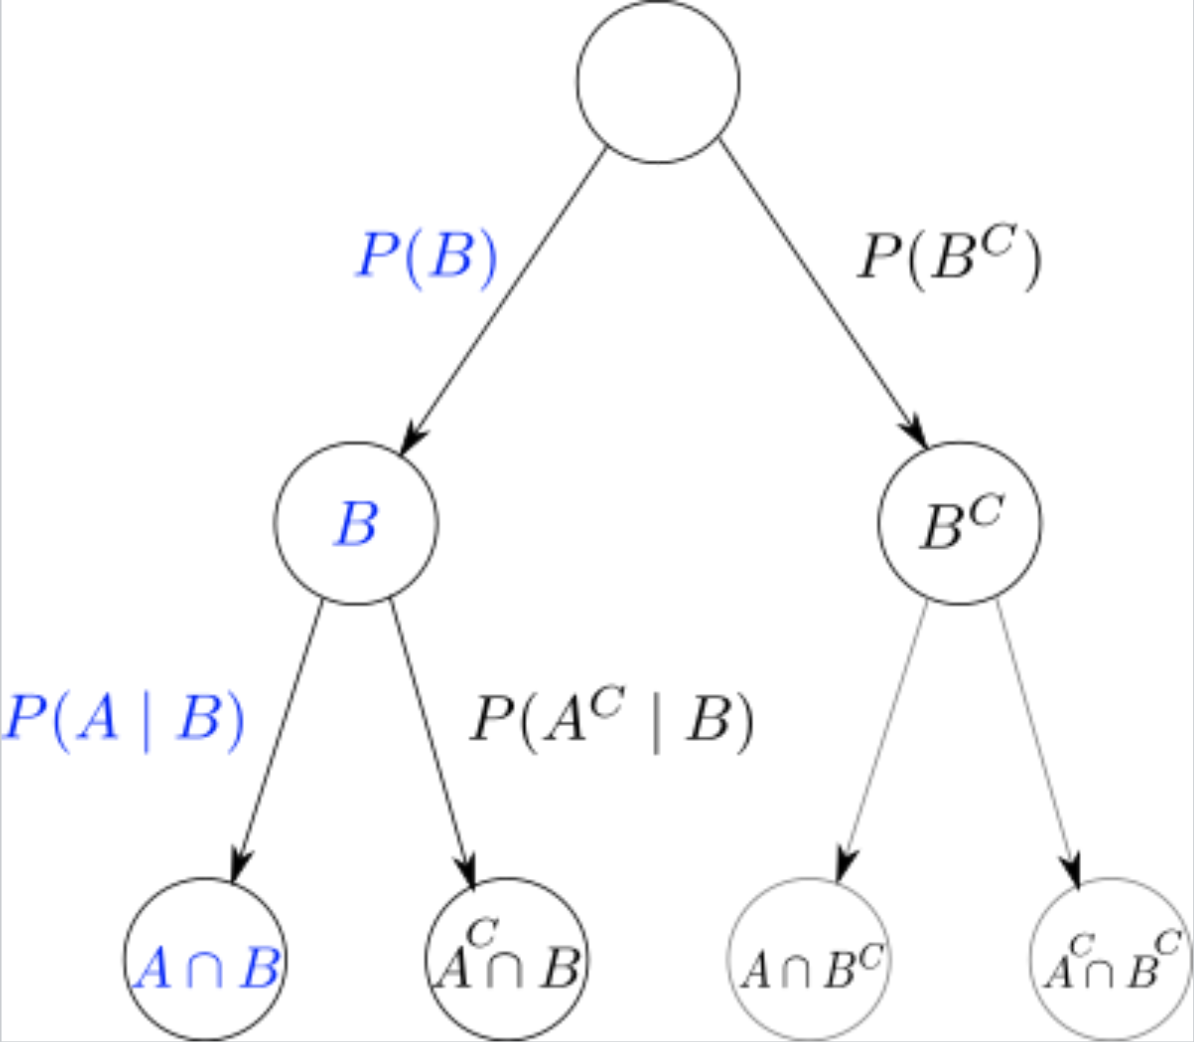
\includegraphics[height=5cm]{figures/tryout.png}
	\caption[Optional optional]{Entscheidungsbaum}
	\label{fig:tryout}
\end{figure}

Wie auf der Abbildung \ref{fig:tryout} zu sehen ist.....


\begin{table}[H]
	\centering
	\label{tab:tryouttab}
\caption[This is an optional caption, without reference]{Local caption, with reference}
	\cite{ref:ds_1, ref:nn_1, ref:ai_1}	% Used to add cites (zitieren)

	\begin{tabular}{l c r}
		Area & Number of rooms & Price \\ \hline
		80	& 4				& 1680 \\
		100	& 5				& 2300 \\
		50	& 2.5				& 1500 \\

	\end{tabular}
\end{table}


\begin{itemize}
	\item This is an item
	\item This is another item
	\begin{itemize}
		\item This is a further item
		\item [blub] This is an item with a custom bullet point
	\end{itemize}
\end{itemize}

\begin{enumerate}
	\item This is a numbered item
	\item And so on
\end{enumerate}


\newpage
\subsection{Math examples}

Here's an example within a sentence $E =mc^2$.

And here one example $$a=v/t$$ which is centred. \\

$$-\frac{\hbar^2}{2m}\frac{d^2\Psi}{dx^2} = E\Psi$$

Fractions

$$d = v_it + \frac{1}{2} \cdot at^2$$
$$d = v_it + \sfrac{1}{2} \cdot at^2$$


Brackets:
$$\left( \frac{1}{2} \right) \cdot 2 = 1$$	% use \left( ..... \right) to match the brackets to the content
$$\left| -7 \right| = 7$$
$$\sqrt{4} = 2$$
$$\sqrt{4} \ne 1$$
$$\sqrt{4} < 5$$
$$ \pi \approx 3 $$
$$ \pi \times \sqrt{4} < 15 $$

\begin{eqnarray}	% Equation array
	3x + 14 &=& 20 \\
	3x &=& 6 \\
	x &=& 2
\end{eqnarray}

\begin{equation}
\label{eq:first}
x^2 + 3x - 7 = 0
\end{equation}

\newpage
\subsection{Graphs}




\begin{tikzpicture}[sibling distance=12em,
							%root/.style={treenode,circle,draw},
							every child node/.style={circle, draw=black},
							]
%	[align=center, sibling distance=5cm]
	\node[fill=black]{}
		child { node {B}
		[sibling distance=6em]
			child { node{A $\cap$ B}  edge from parent node[left] {$P(A|B)$} }
			child { node{$\bar{A} \cap B$} edge from parent node[right] {$P(\bar{A}|B)$}}
			}
		child{ node{$\bar{B}$}
			[sibling distance=6em]
			child{ node{$A \cap \bar{B}$} edge from parent node[left] {$P(A|\bar{B})$}}
			child{ node{$\bar{A} \cap \bar{B}$} edge from parent node[right] {$P(\bar{A}|\bar{B})$} }
		       }
	;

\end{tikzpicture}
% ****************************************************************

% ============================================================




% REFERENCES ============================================================
\cleardoublepage
%\renewcommand{\bibname}{Referenzen}	% Rename the bibliography title
\bibliographystyle{IEEEtran}	% Adds cites (Zitate)
\addcontentsline{toc}{section}{Referenzen}
% references can easily be generated using the OS X tool "BibDesk"
% Make sure you build your LaTeX document in BibTeX after defining your references
%	in order to make them valid.
\bibliography{references/book_ref1}
% ============================================================

% APPENDIX ============================================================
\cleardoublepage
\appendix
\section{Cheatsheet}
% ============================================================


\end{document}